\chapter{Perspectives}

In this thesis we introduced the \HubLem fragmentation model and applied to the dynamical evolution of substructured star clusters and the fate of their binary population. Interesting results have been obtained, though some assumptions were made. In this chapter, we review two of these assumptions: the absence of stellar evolution and the isolated nature of the cluster. We also present the outline of a comparison to observations and the possible inclusion of hydrodynamical processes.






\section{Tidal field}

In all our simulations, it was assumed the clusters were in isolation and no tidal field were applied. This allowed to study the mechanisms of violent relaxation and the erasure of substructure. However, in reality, star forming regions are shaped by the gravitational influence of their surroundings. We mentioned in section \ref{Sec:2_conclusion} that the galactic tidal field could prevent the collapse of the \HubLem fragmented configuration and scatter the clumps, injecting them in the galactic cluster mass function. The fate of these clumps is uncertain, as some will disperse through two-body interactions, and other will merge, depending on the geometry imposed by the tidal field. 

Numerical simulations will allow an exploration of the resulting clump mass function, which would be more directly comparable to the cluster mass function. NBODY6 has a built-in galactic tidal field module, which allows to model the tidal forces associated with the cluster orbiting a complex galactic potential, including a \cite{Miyamoto1975} potential, see \cite{Aarseth2003} for details. The tidal shock from a passing molecular cloud is also an option in NBODY6.

However, it is possible to go further in the inclusion of realistic tidal fields. \cite{Renaud2011} introduced a new version of NBODY6, \href{http://personal.ph.surrey.ac.uk/~fr0005/nbody6tt.php}{Nbody6tt}, that can take an arbitrary tidal tensor as an input and apply it to the evolution of a star cluster. Specifically, Nbody6tt allows to extract the tidal environment of a cluster from a large-scale galactic simulation to obtain a time-dependant, self-consistent tidal field. The influence of different galactic environment, such as tidal arms, on the cluster can then be evaluated. 

For example, \cite{Renaud2015b} reported the formation of massive clusters in their hydrodynamical simulation of a galaxy merger analog to the Antennas galaxies. Fig~\ref{Fig:7_renaud} show the merging of YMC fragments on large scales. This kind of event could be reproduced in Nbody6tt with a \HubLem configuration and the tidal data from the simulation. Given the complex tidal fields in this kind of environment, the evolution of YMCs starting from a substructured initial conditions could shed light of their formation and disruption processes.


\begin{figure}
\begin{center}
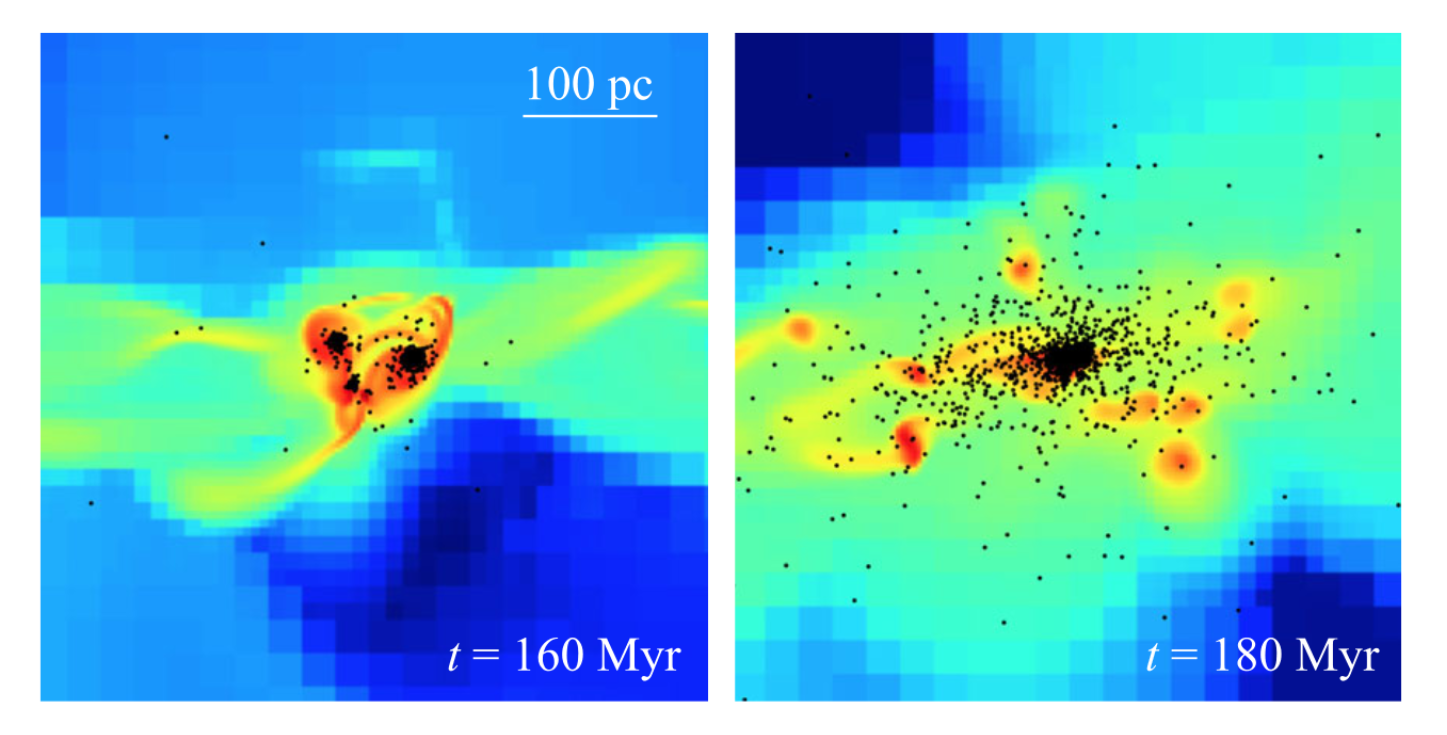
\includegraphics[width=0.7\textwidth]{Figures/7_renaudantennas.png}
\end{center}
\caption{Cluster formation in a hydrodynamical simulation of the Antennaes galaxies. The colormap indicates gas densities and newly formed stars are shown as black dots. Two epochs are shown, outlining the erasure of substructure. The figure was extracted from \cite{Renaud2015b} }
\label{Fig:7_renaud}
\end{figure} 



\section{Stellar evolution}

In section \ref{Sec:3_Scaling} and TODO, we selected the mass ranges to apply to our models, which we justified by the duration of our simulations, arguing the death of our most massive stars would either not happen or not have a significant impact on the evolution. However, in section TODO, we remarked that the inclusion of even more massive stars could be of interest for the formation of new tight binaries.

It comes that one of the most straightforward ways to improve our models is the inclusion of stellar evolution. NBODY6 has a built-in stellar evolution module based on the analytical mode by \cite{Hurley2000}, including wind-driven mass loss, radii evolution, supernova event and stellar remnants. It was not used in this work for simplicity, but should be used for further research.


In section TODO, we computed free-fall times for models with several initial stellar densities. This corresponds to the lifetimes of clumps, as the collapse and relaxation erase substructure. We then ask to what extent the death of massive stars can affect the dynamics of a single clumps. From \cite{Hurley2000}, we get stellar lifetimes as a function of mass, shown on Fig~\ref{Fig:7_stellarlifetime}. For low stellar density, clumps can barely outlive massive stars. We showed that for an initial stellar density of 6 stars/$\pc^{-3}$, the system collapses in 6 Myr, while stars with a mass $> 10 \Mo$ live up to 5 Myr.

However, if we include tidal fields, the clumps might survive far longer, and the mass-loss from stellar evolution could have a significant impact on their structures, their mass segregation, and  on the overall clump mass function.


\begin{figure}
\begin{center}
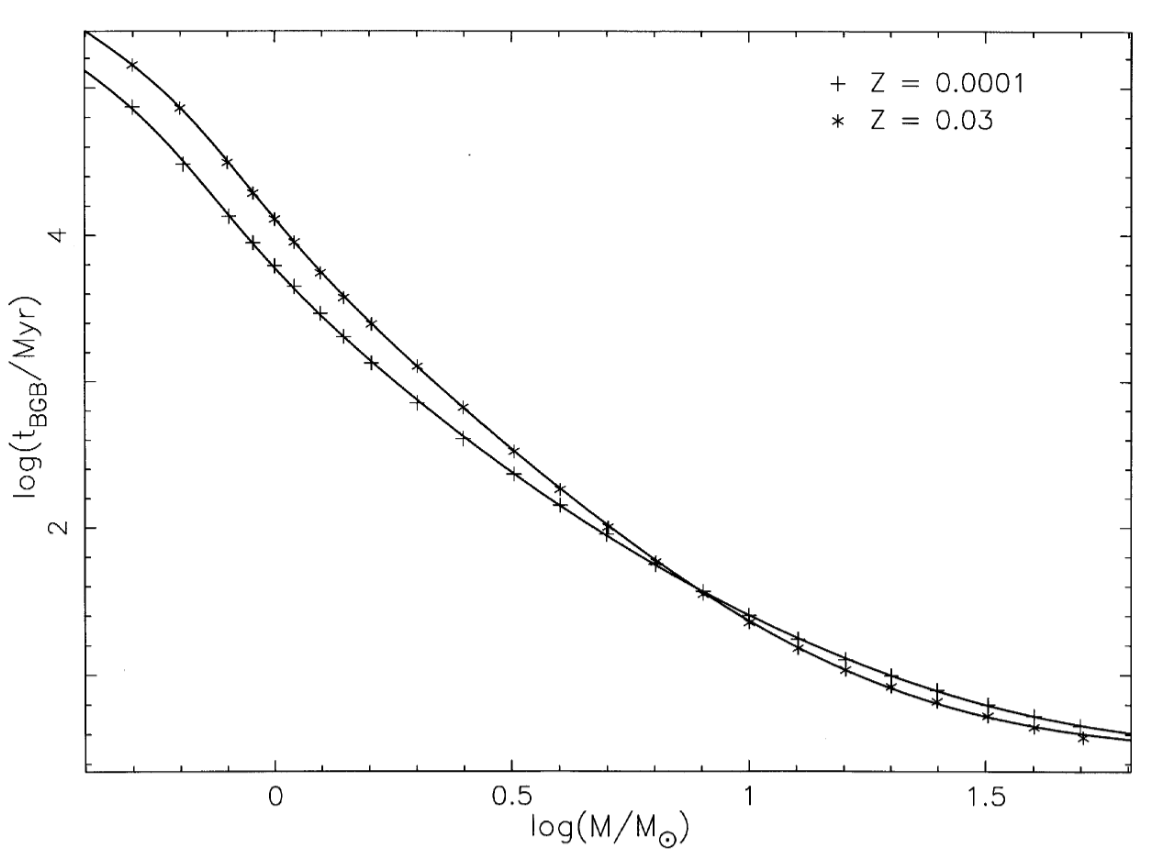
\includegraphics[width=0.7\textwidth]{Figures/7_stellarlifetime.png}
\end{center}
\caption{Time taken to reach the Base of the Giant Branch (BGB) as a function of initial stellar mass, for two metallicities, Z = 0.0001 and Z = 0.03. The figure was extracted from \cite{Hurley2000}}
\label{Fig:7_stellarlifetime}
\end{figure} 



\section{Anisotropic expansion}

The \HubLem expansion we used throughout this thesis was isotropic, the velocity field was expressed with $\bold{v} = \Hub_0 \bold{r}$ with \tHub a scalar value. As a result, the fragmented configurations are roughly spherical and the net systemic angular momentum is null. This is a key difference between the method we have developed and the fractal approach of \cite{Goodwin04}. Angular momentum may be significant in young clusters such as R136 \citep{Henault-Brunet2012}. In a fractal model, the way the velocity field is built leaves a residual, global angular momentum whereas the Hubble approach starts off with strictly zero angular momentum.

 A net angular momentum could be introduced in a Hubble model, for instance by setting 
\begin{equation}
\bold{v} = \Hub_o \bold{r} + \bold{\Omega} \times \bold{r}
\end{equation} 
with $\bold{\Omega}$ a chosen angular velocity. One can actually go further and write in matrix form
\begin{equation}
\bold{v} = \bold{H}\bold{r},
\end{equation}
with $\bold{H}$ now a 3$\times$3 matrix, where the off-diagonal elements account for rotation and the elements on the diagonal $\Hub_{ii}$ control the three dimensional expansion. In this study, we have set $\Hub_{ij,i\ne j}=0$ and $\Hub_{ii}=\Hub_o$ otherwise. It is then a simple matter to study the fragmentation along a filament by setting, for example, $\Hub_{xx}=\Hub_{yy}=0$ and $\Hub_{zz}>0$. The Hubble fragmentation process for young stellar cluster is a new method and many of its aspects remain to be explored.


 As mentioned earlier, recent observations confirmed the prevalence of filamentary structure in star formation processes \citep{Andre2010}. 



